\chapter{Data Preparation \& Model Training} \label{chap:training}

\section{Introduction}
The PU-Net and RNN networks provide a powerful way to learn the electronics response. Ideally, the ATN should be trained with paired waveforms of simulations and data. In reality, collecting such a paired dataset is a big challenge. Although we can simulate $\mathcal{T}_{Source}$ from an arbitrary $\mathcal{D}_{Source}$, obtaining a corresponding $\mathcal{T}_{Target}$ such that $\mathcal{D}_{Source} = \mathcal{D}_{Target}$ is difficult without precise knowledge of $P(X'|Y')$. Consequently, training must be performed on unpaired datasets, where $\mathcal{D}_{Source} \neq \mathcal{D}_{Target}$. The CycleGAN framework~\cite{CycleGAN} provides an unsupervised learning approach to train the ATN using adversarial losses. We call this model combining all the Cyclic Positional U-Net (CPU-Net). CPU-Net was originally developed by Aobo Li.

In this chapter, we describe the CPU-Net training process. First, we outline the detector data collection and processing. Then, we discuss how we obtained the simulation dataset. Finally, we detail the training of the network using CycleGAN.

\section{Data selection}

The LEGEND Collaboration characterizes newly produced HPGe detectors at Oak Ridge National Laboratory (ORNL). We used characterization data from a LEGEND Inverted-Coaxial Point-Contact (ICPC) detector, V06643A, manufactured by ORTEC. The detector was mounted in a PopTop configuration, surrounded by lead shielding, and placed in a concrete alcove to reduce the external background. The data contained a flood Thorium-232 source on top of the detector. The detector signals were digitized using a FlashCam digitizer and the \texttt{pygama} package~\cite{pygama} was used to convert the FlashCam output to LEGEND HDF5 files.  The event energies were calibrated to convert the ADC units to keV. The energies were then corrected for charge trapping. The left panel of Figure~\ref{ch7_fig_eng_spec_comp} shows the final energy spectrum obtained from the detector.

The escape peaks in the spectrum are created from pair production events from a high-energy photon. In this process, the incident photon generates an electron-positron pair. The electron is collected by the detector, while the positron quickly annihilates, producing two additional gamma-ray photons. If all secondary gamma rays are fully absorbed within the detector, their combined energy yields a characterized peak in the energy spectrum, the Full Energy Peak (FEP).

If one of the annihilation gamma rays leaves the detector without depositing its energy, the spectrum shows a Single Escape Peak (SEP). This scenario results in a multi-site (MS) event because the signal comprises two distinct interactions within the detector: the collection of the pair-produced electron and the absorption of one of the two gamma rays. If both gamma rays escape the detector without interaction, a double escape peak (DEP) is observed. This situation corresponds to a single-site (SS) event since the only interaction that contributes to the signal is the collection of the pair-produced electron. Tl-208 is part of the decay chain of $^{228}$Th and produces an FEP at $2614.53$ keV. Given that the mass of the electron is $511$ keV, the SEP peak occurs at $2103.53$ keV and the DEP peak at $1592.53$ keV. 


\begin{figure}%[htb!]
  %[trim={left bottom right top},clip]
    \centering
    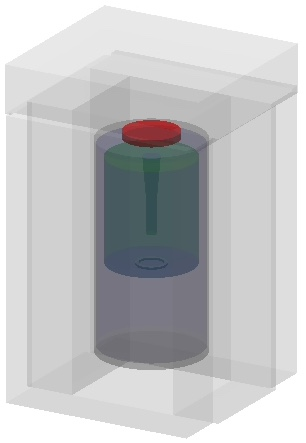
\includegraphics[width=0.4\linewidth]{ch7/figs/shielding.jpeg}
    \caption{The simulation geometry of the ORNL characterization setup, showing the detector in green, the source in red, the aluminum holder in light blue, and the lead shielding in light grey.}
   \label{ch7_fig_g4simple_setup}
\end{figure}


\begin{figure}%[htb!]
\centering
  %[trim={left bottom right top},clip]
    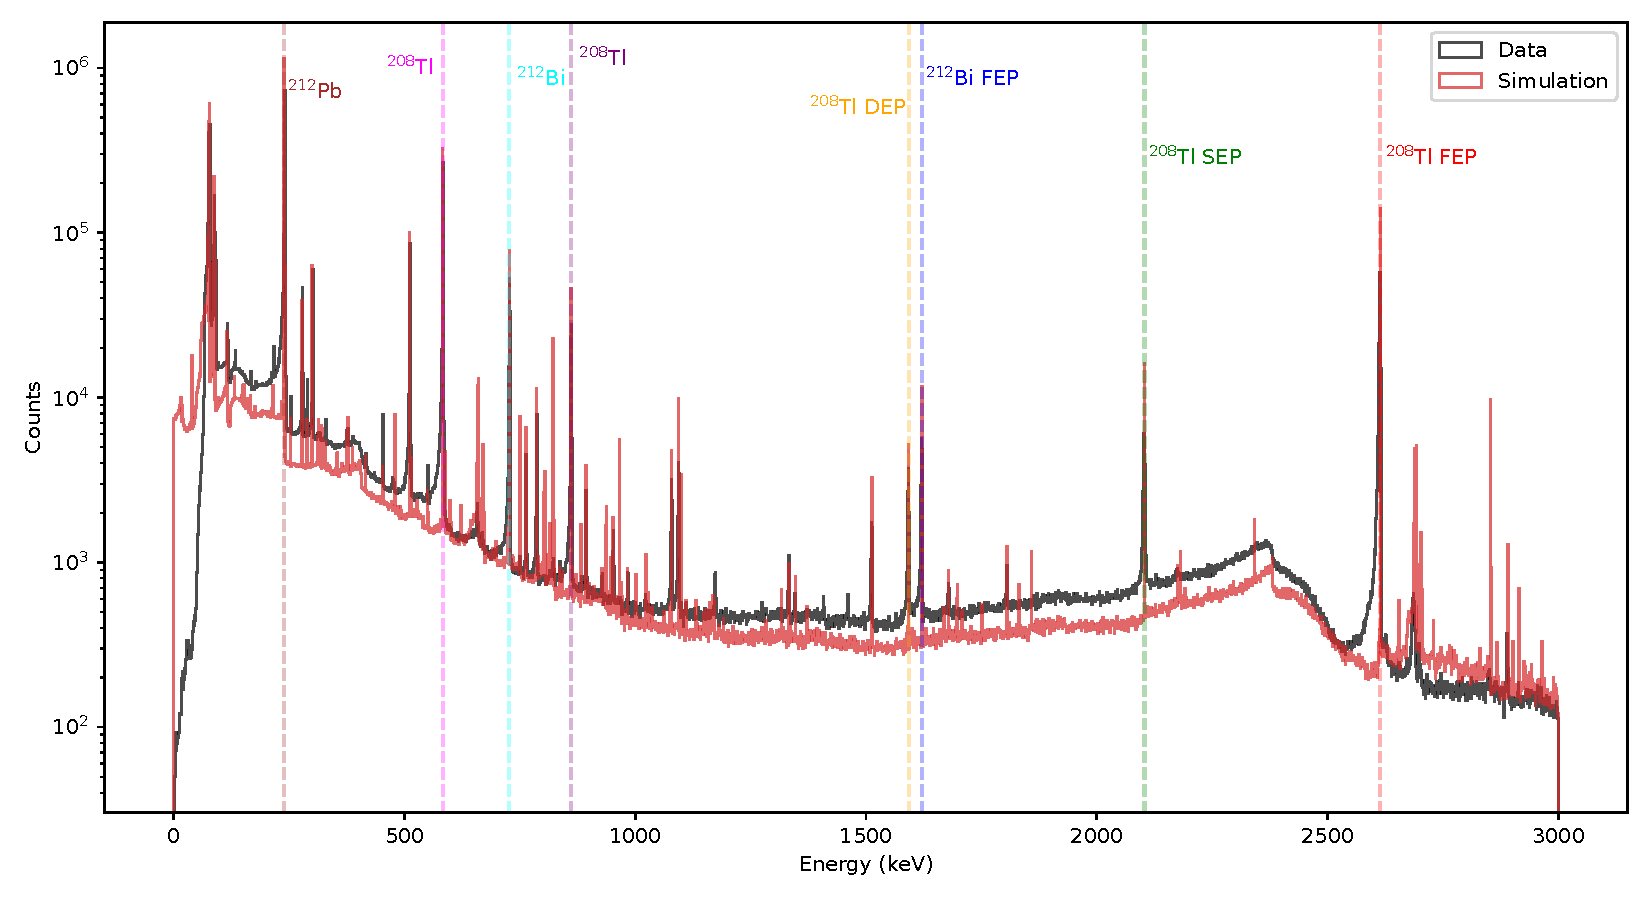
\includegraphics[width=0.99\linewidth,trim={0pc 0pc 0pc 0pc},clip]{ch7/figs/energy_spectrum_comparison.pdf}
    \caption{Calibrated energy spectrum from a $^{228}$Th source at ORNL compared to the Monte Carlo simulation results. Key peaks from $^{228}$Th source are labeled.}
   \label{ch7_fig_eng_spec_comp}
\end{figure}

\section{Simulations}
We designed a simple Geant4 setup geometry to simulate events in the ORNL characterization setup. The setup in Geant4 is shown in Figure \ref{ch7_fig_g4simple_setup} This includes a Germanium detector, a radioactive source, an Aluminum PopTop cryostat holder, surrounded by lead shielding. We simulated 100 million $^{228}$Th decay events originating from the source and recorded their energy depositions within the germanium detector. Given the location of energy deposition within the detector, we used {\siggen} simulations to generate waveforms for hits in the DEP, SEP, and FEP energies.

Waveforms for multi-site events are created by energy-weighted summing of individual hits waveforms. Figure ~\ref{ch7_fig_eng_dep_sim} shows the simulation process for a few events. The left panel depicts the hit locations of the particles for the events. Event 3 and Event 4 are effectively single-sited, as the energy depositions occur very close to each other, and thus produce single-sited events. In Event 1, the energy depositions result in two primary sites, giving rise to a two-sited waveform. Event 2 features a trace of energy deposition localized to three regions, which is classified as a three-site event. Events 3 and 4 have different drift times because they are deposited at different distances from the point contact.

\begin{figure}[htb!]
  %[trim={left bottom right top},clip]
    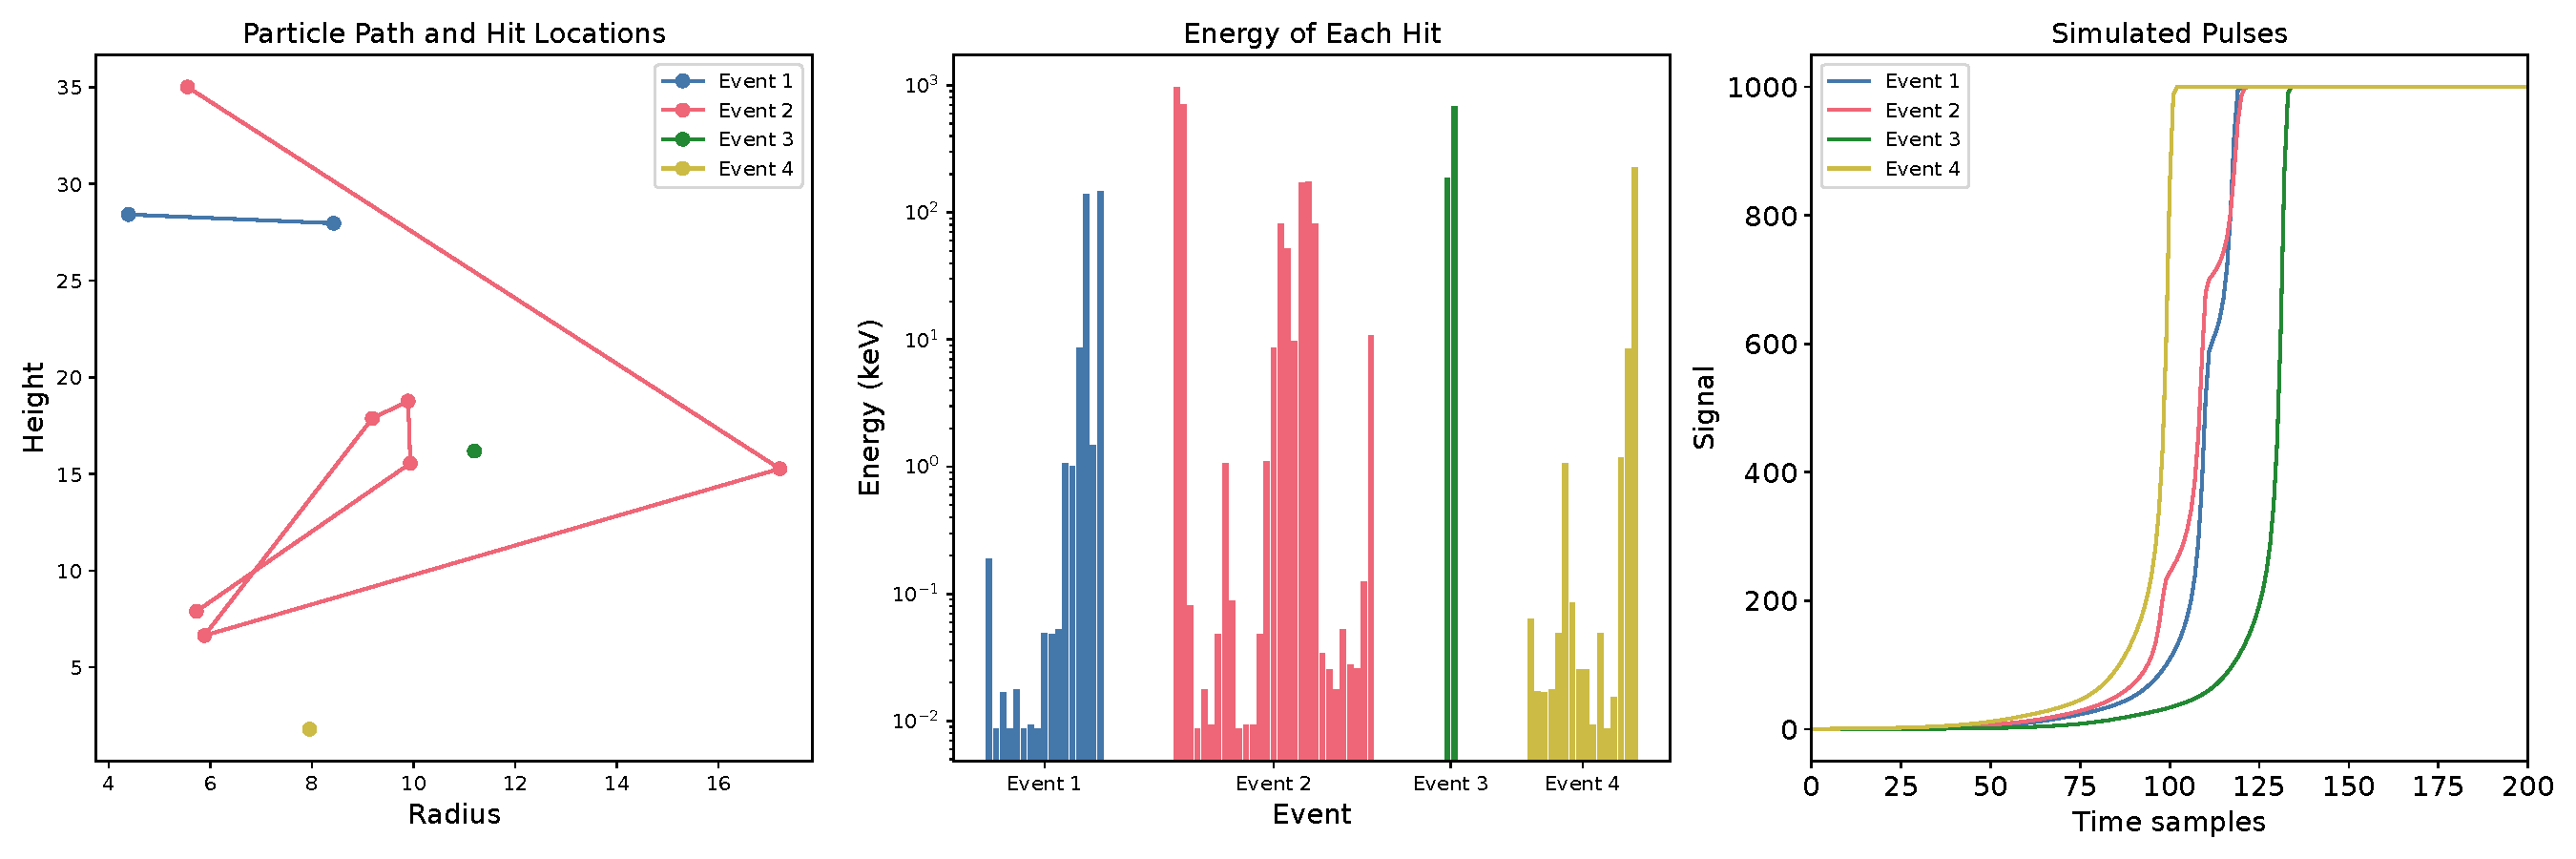
\includegraphics[width=0.99\linewidth,trim={1pc 0pc 1pc 0pc},clip]{ch7/figs/hit_sims.pdf}
    \caption{Production of energy weighted waveform in simulations for 4 events. Left figures show the location of hit locations for each event.  The magnitude of energy deposited for hits in each event is shown in middle figure. Right figure show the energy-weighted waveforms for the corresponding events. Hits produced using \texttt{Geant4} simulations and waveforms are generated using {\siggen} software.}
   \label{ch7_fig_eng_dep_sim}
\end{figure}


\section{Post Processing}

Normalizing and aligning the waveforms are crucial for training the network. The sim waveforms are already normalized between 0 and 1. The raw data waveforms are normalized by dividing by the $80\%$ of the average of the last five samples. The waveform is then vertically shifted so that the average of the first 200 samples is zero. This ensures that all waveforms have their RC decay tails and baseline aligned, which can help the model learn the features better. Then we used the $99.9\%$ rise time to horizontally align the waveform. We found that this method was more effective in training the network than aligning by the zero time point. The waveforms are padded to ensure that there are 400 samples on both sides of the $99.9\%$ rise time. The tail slope $\tau$ is calculated by the slope of a linear fit of the logarithm of the last 300 waveform samples. Events with poor fit quality $\chi^2$ or anomalous $\tau$ are used to identify pile-up waveforms and remove them from the training. Figure \ref{ch7:figs:in_out} shows the processed data and sim waveforms that are fed into the neural networks.

\begin{figure}%[!htb]
    % \hspace{0.05\linewidth}
    %[trim={left bottom right top},clip]
    \centering
    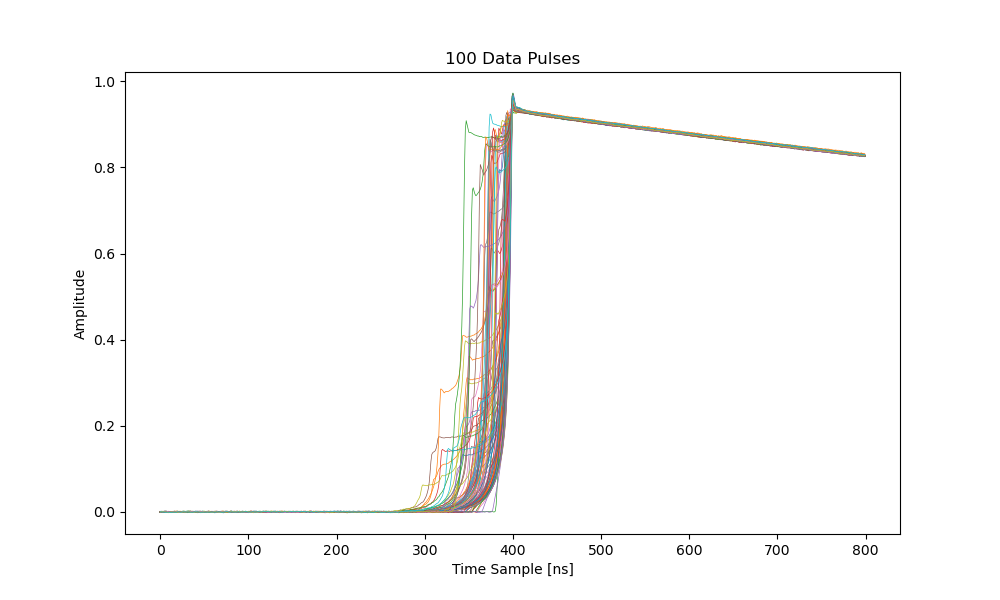
\includegraphics[width=0.9\linewidth,trim={4pc 0cm 6pc 1cm},clip]{ch7/figs/all_data_pulses.png}
    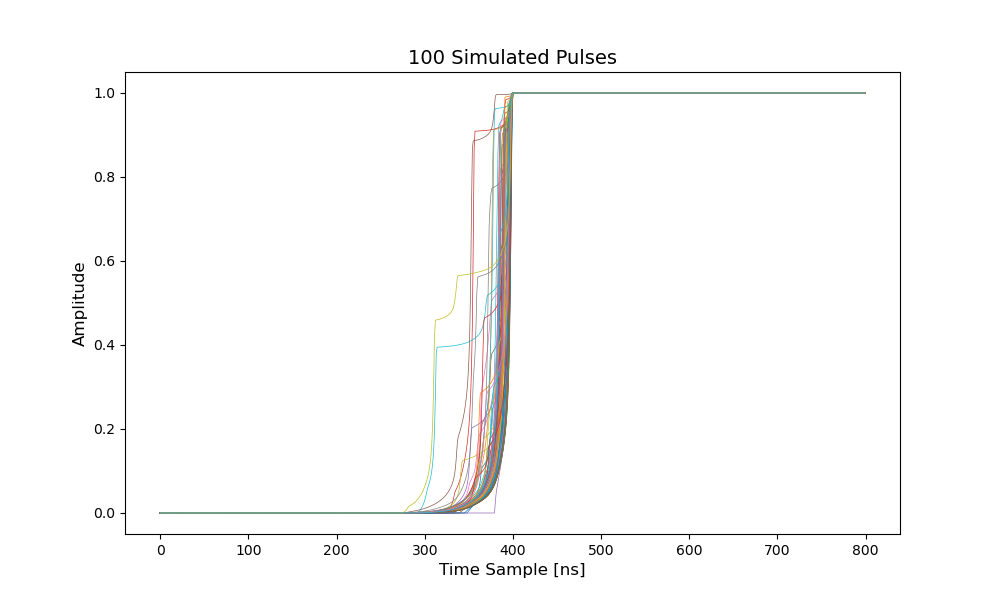
\includegraphics[width=0.9\linewidth,trim={4pc 0cm 6pc 1cm},clip]{ch7/figs/all_simulated_pulses.png}
    \caption{Input data and simulated waveforms. The waveforms are aligned by $99.9\%$ rise time. Data pulses are normalized by aligning the tail and baselines.}
   \label{ch7:figs:in_out}
\end{figure}

\section{Network Training}

The training and validation of CPU-Net is conducted in PyTorch~\cite{pytorch}. We construct two networks, an ATN~ $\Lambda$ and an inverse ATN $\bar{\Lambda}$, both with the PU-Net structure. We then construct two RNN discriminator networks: sim discriminator $\delta_{S}$ and data discriminator $\delta_{T}$ for the source and target waveforms, respectively. Figure~\ref{fig:network_training} shows the overall training process.
\clearpage
\begin{figure}[htb!]
    \centering
    % \hspace{0.05\linewidth}
    %[trim={left bottom right top},clip]
    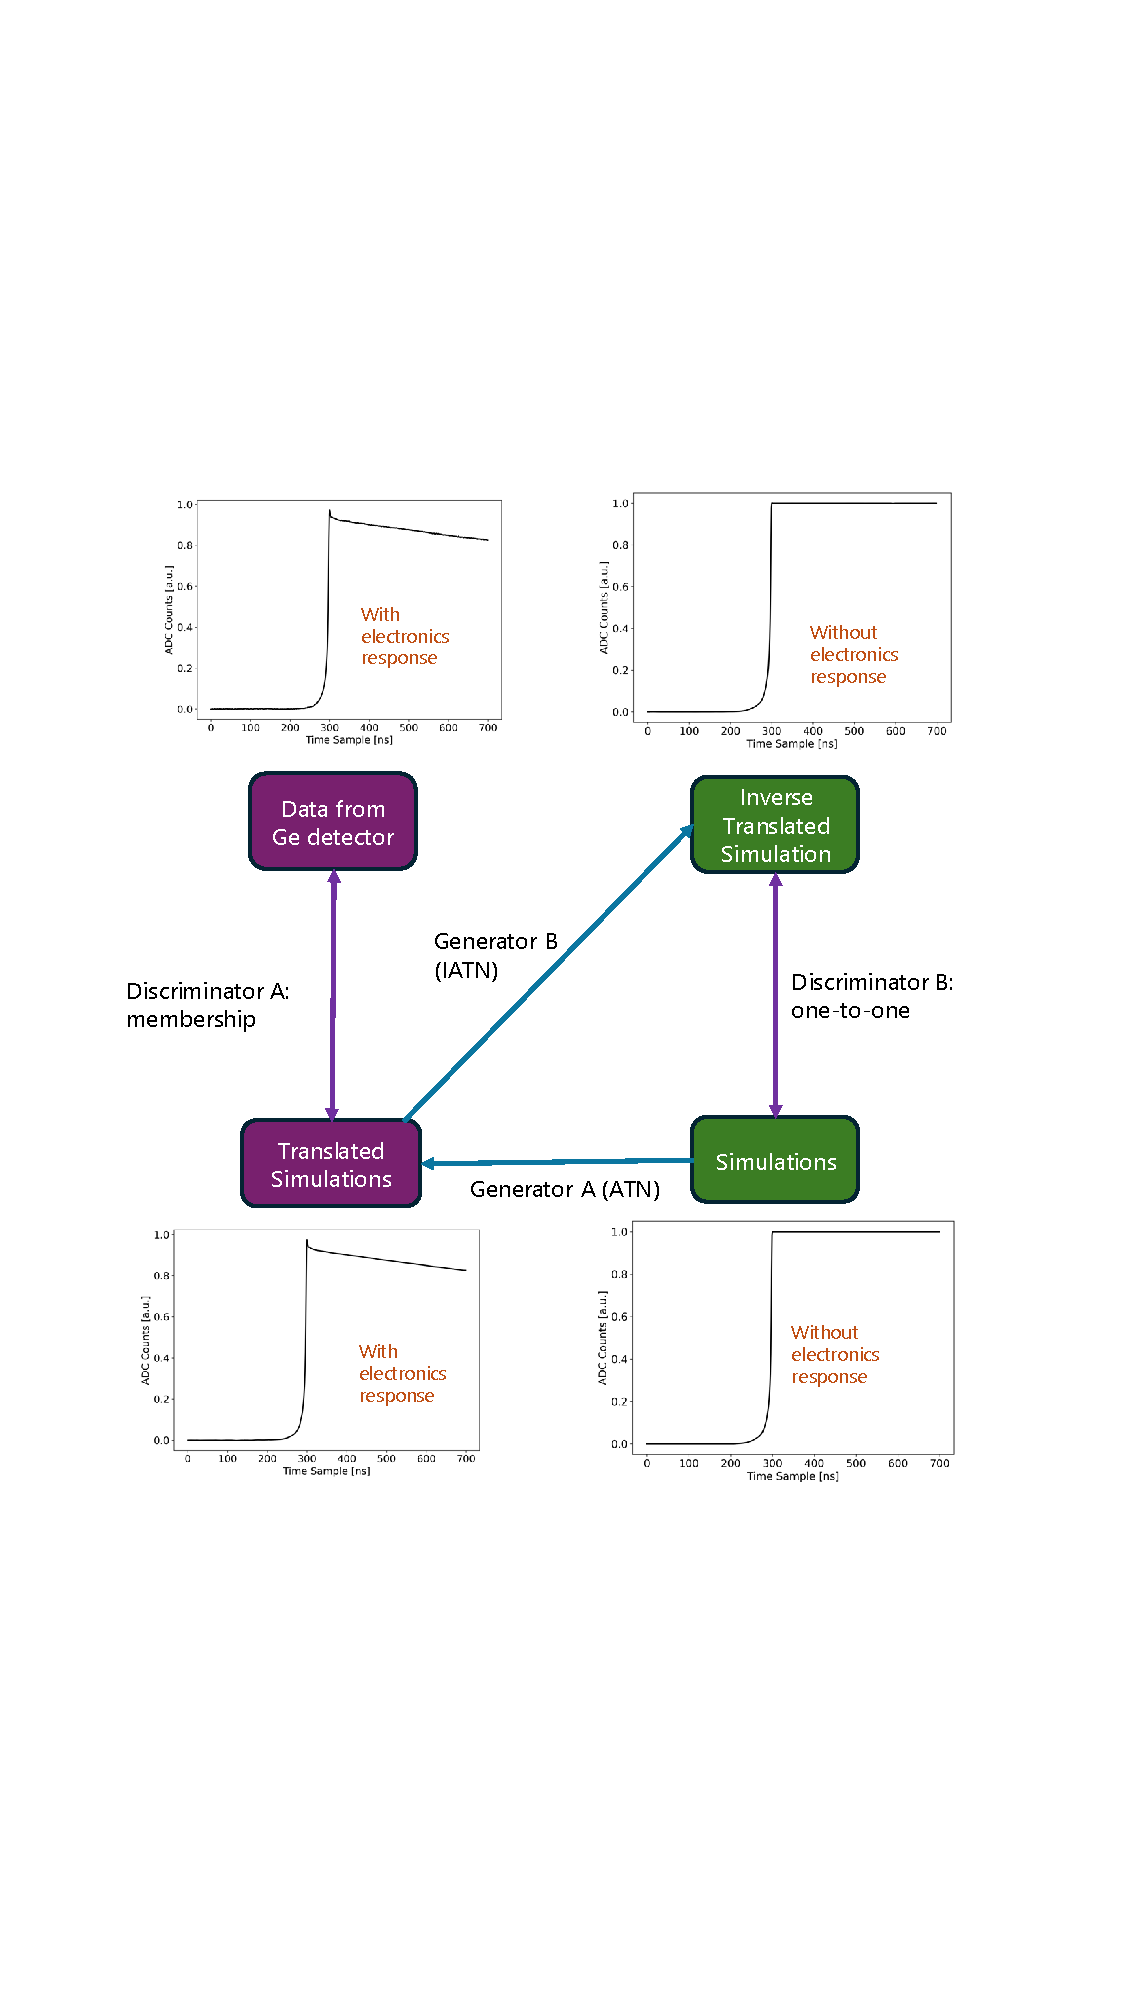
\includegraphics[width=0.99\linewidth,trim={5.5pc 20pc 6.3pc 19pc},clip]{ch7/figs/cycle_gan_training.pdf}
    \caption{Training in CPU net. ATN transfers simulation to data like while IATN transfers data to simulation. Discriminator A differentiates data like waveform output ATN from data. Discriminator B differentiates simulation like waveform output IATN from simulations.}
   \label{fig:network_training}
\end{figure}


During training, a simulated waveform $X$ is first fed to $\Lambda$ to produce a translated waveform $\Lambda(X)$. The discriminator $\delta_{T}$ attempts to distinguish $\Lambda(X)$ from real data waveforms while $\Lambda(X)$ attempts to `fool' $\delta_{T}$. Then $\Lambda(X)$ is fed to $\bar{\Lambda}$ to translate back to $\mathcal{X}$ space by $\bar{\Lambda}(\Lambda(\mathcal{X}))$. A second discriminator $\delta_{S}$ attempts to distinguish $\bar{\Lambda}(\Lambda(\mathcal{X}))$ from $\mathcal{X}$, while $\bar{\Lambda}$ attempts to `fool' $\delta_{S}$. The $\mathcal{X}\rightarrow{}\Lambda(\mathcal{X})\rightarrow{}\bar{\Lambda}(\Lambda(\mathcal{X}))$ translation path is termed the forward cycle. The same process is performed in the other direction, starting with the detector waveform $\mathcal{X}'\rightarrow{}\bar{\Lambda}(\mathcal{X}')\rightarrow{}\Lambda(\bar{\Lambda}(\mathcal{X}'))$ and called the backward cycle.

\section{Loss Functions}

Since there is no direct comparison loss, we define three losses that are optimized during training to help the network learn the translations. $L_{\mathrm{Identity}}$ ensures that the ATN retains its shape when a actual detector waveform $X'$ is fed into $\Lambda$, shown in the equation. \ref{eq:loss_ided}. The cycle-consistent loss in Equation \ref{eq:loss_cyc} ensures that the circular translation path preserves the original waveform shape. 

In both cycles and identities, the waveform is compared with another waveform. For such a comparison, we define a specialized L1 loss that emphasizes different parts of the waveform by assigning them varying weights. It is designed to give more importance to the rising and falling edges of the waveform, which are critical for accurate pulse shape analysis.

The GAN loss Equation \ref{eq:loss_gan} calculates the loss associated with `fooling' the discriminator.  The discriminators output a single value between 0 and 1. A value close to 1 means that the discriminator classifies it as data, while a value 0 close to zero means that the discriminator classifies it as simulation. Binary cross-entropy loss is used to quantify the performance of the discriminators $\delta_{T}$ and $\delta_{S}$. The loss calculations are summarized in Table \ref{ch8_tab_loss_summary}.

\begin{equation}\label{eq:loss_ided}
    L_{\mathrm{Identity}} = |X' - \Lambda(X')|
\end{equation}
\begin{equation}\label{eq:loss_cyc}
    L_{\mathrm{Cycle}} = |X - \bar{\Lambda}(\Lambda(X))|
\end{equation}
\begin{equation}\label{eq:loss_gan}
    L_{\mathrm{Adversarial}} = E_{\mathcal{X'}}\log(\delta(X')) - E_{\Lambda(\mathcal{X})}\log(1 - \delta(\Lambda(X)))
\end{equation}

An additional three complementary losses are defined for the detector waveform translation path. Therefore, a total of six losses are optimized simultaneously for the generators and two for the discriminators.  

\begin{table}%[ht!]
\centering
\renewcommand{\arraystretch}{1.5} % Adjust row height for readability
\setlength{\tabcolsep}{2.0pt} % Adjust column spacing
\begin{tabular}{|p{0.18\linewidth}|p{0.39\linewidth}|p{0.22\linewidth}|p{0.15\linewidth}|}
\hline
Loss                & Calculation                             & Type of Loss                                  & Optimizer   \\ \hline
Identity Losses    & Data - ATN(Data)                                & \multirow{3}{=}{Custom L1 Loss} & \multirow{8}{=}{Optimizer 1} \\
                             & Sim - IATN(Data)                                 &                                                       &                       \\ \cline{1-3}
Cycle Losses        & Data – ATN(IATN(Data))                         & \multirow{3}{=}{Custom L1 Loss} &                       \\
                             & Sim – IATN(ATN(Sim))                          &                                                       &                       \\ \cline{1-3}
Generator Losses    & Disc B (IATN(Data))                              & \multirow{2}{=}{Binary Cross Entropy}                &                       \\
                             & Disc A (ATN(Sim))                              &                                                       &                       \\ \hline
Discriminator A     & {[Disc A(Data) - 1]} + {[Disc A(Sim) - 0]}        &  Binary Cross Entropy                                & Optimizers 2 \\ \hline
 Discriminator B    & {[Disc B(Sim) - 1]} + {[Disc B(Data) - 0]}        &   Binary Cross Entropy                                &   Optimizers 3             \\ \hline
\end{tabular}
\caption{Overview of Loss Calculations, Loss Types, and Optimizers.}
\label{ch8_tab_loss_summary}
\end{table}


AdamW~\cite{adam_w_paper} optimizers are used for all losses. Compared to the traditional Adam optimizer, AdamW applies weight decay as a separate step during gradient descent optimization. This avoids interference with the learning rate schedule and helps stabilize the training process. In total, we define three optimizers shown in the table.\ref{ch8_tab_loss_summary}. The six losses for ATN and IATN are optimized together, and the discriminators each have their own optimizers.


% Combining all these, we obtain the Cyclic Positional U-Net~(CPU-Net) for Ad-hoc waveform shape simulation.
\section{Hyperparameter Tuning}
Achieving stability in CycleGAN training can be challenging. This is because the loss optimization process is complex as there is not one metric such as mean squared difference being optimized. Training must balance the learning progress of generators and discriminators while preventing gradients from exploding or imploding to zero. To improve training, we introduced hyperparameters at different levels of the model that are summarized in Table \ref{tab:hyperparameters}.

\begin{table}%[htb!]
\centering
\renewcommand{\arraystretch}{1.5} % Adjust row height for readability
\setlength{\tabcolsep}{2pt} % Adjust column spacing
\begin{tabular}{|p{0.18\linewidth}|p{0.12\linewidth}|p{0.65\linewidth}|}
\hline
\textbf{Hyperparameter}       & \textbf{Value} & \textbf{Description} \\ \hline
batch\_size          & 32             & Number of pulses used in one training iteration. \\ \hline
baseline\_len        & 200            & Number of samples assigned to baseline portion of the waveform. \\ \hline
rising\_edge\_len    & 250            & Number of samples assigned to the rising edge of the waveform. \\ \hline
tail\_len            & 350            & Number of samples assigned to the RC decay tail of the waveform. \\ \hline
baseline\_weight     & 3.0            & Weight given to baseline portion of the waveform in the loss. \\ \hline
ris\_edge\_weight    & 10.0           & Weight given to rising edge portion of the waveform in the loss. \\ \hline
tail\_weight         & 7.0            & Weight given to RC decay tail portion of the waveform in the loss. \\ \hline
iters                & 7000           & Maximum number of iterations for training. \\ \hline
decay                & 1000           & Iteration at which learning rate starts to decay. \\ \hline
lrate\_gen           & $1 \times 10^{-3}$ & Learning rate for the generator networks. \\ \hline
lrate\_disc          & $1 \times 10^{-3}$ & Learning rate for the discriminator networks. \\ \hline
cyc\_loss\_weight    & 20             & Weight of the cycle consistency losses.  \\ \hline
iden\_loss\_weight   & 5              & Weight of the identity loss. \\ \hline
gan\_loss\_weight    & 9              & Weight of the generator loss. \\ \hline
max\_grad\_norm      & 100            & Maximum gradient norm for gradient clipping. \\ \hline
w\_decay             & $1 \times 10^{-4}$ & Weight decay in the optimizers. \\ \hline
n\_disc\_iters       & 30             & Number of iterations after which the discriminators are updated. \\ \hline
\end{tabular}
\caption{Hyperparameters used for CPU-Net training.}
\label{tab:hyperparameters}
\end{table}


It was found that the discriminator typically overpowers the generator, since the generator has a more complex task of generating waveforms while maintaining the cycle and identity consistency and also fooling the discriminator. To balance this, we update the weights of the generators more frequently than the discriminators. We introduced a hyperparameter for the number of intervals after which the discriminator is updated. This allowed the generator enough steps to adapt to changes in the discriminator without destabilizing the adversarial process.

The weighting of the adversarial, cycle-consistency, and identity losses enables fine-tuning the learning of the generators. At some point, the generator would have learned just enough to fool the discriminator, and further learning might be hampered. The loss weights are used to emphasize the generator to learn translation, such as the cycle and identity consistency even if it has been successful at overpowering the discriminator. These hyperparameters are carefully tuned to achieve a balance, as values that are too high will cause the gradient to explode; too low will cause the model to not learn much. 

We also introduced a learning rate decay for the optimizers. In the beginning, the learning rate is intentionally kept high for the model to explore the entire parameter space, then the learning rate decays linearly to help it converge in the right direction. This is particularly important for the ATN optimizer, as it is optimizing six losses, and this ensures that all the space is explored.

To prevent overfitting during training, weight decay is applied to the optimizers so that it penalizes the large weights and ensures generalization among all parameters. Gradient clipping is applied, limiting the norm of gradients during training and preventing exploding gradients, particularly in layers of the U-Net. The threshold for clipping the magnitude of gradients is kept high, since the loss is multiplied by different loss weights multiple times, which can increase the magnitude.

Together, these parameters enable price fine-tuning CPU-Net training to obtain the right balance during training. A single training takes about 1 GPU hour on a NVIDIA A100 GPU. The trained CPU-Net generates both an ATN and an inverse ATN, which enable bidirectional translation between the simulation and data domains. The ATN is the primary focus of this work, but the reverse ATN can also enhance analysis by refining the waveform reconstruction. In the next chapter, we discuss some results from the ATN output.